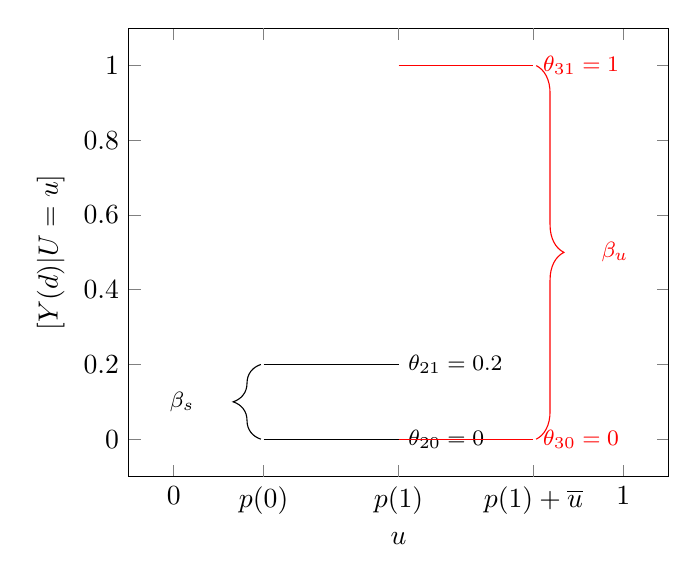
\begin{tikzpicture}
	\begin{axis}[
		xmin=-0.1, xmax=1.1,
		ymin=-0.1, ymax=1.1,
		xlabel=$u$,
		ylabel={$\E[Y(d)|U=u]$},
		xtick={0,1}, % Specify the x-axis ticks here
		extra x ticks={0.2, 0.5, 0.8}, % Specify the positions of the special x-axis ticks together
        extra x tick style={xticklabel style={color=black}}, % Apply a style to all extra x ticks
        extra x tick labels={$p(0)$, $p(1)$, $p(1) + \overline{u}$}, % Customize the labels of the special x-axis ticks
    ]

	\addplot [domain=0.2:0.5, color=black] {0} node[pos=1, right] {\footnotesize $\theta_{20} = 0$};
	\addplot [domain=0.2:0.5, color=black] {0.2} node[pos=1, right] {\footnotesize $\theta_{21} = 0.2$};

	\draw [decorate,decoration={brace,amplitude=10pt,raise=0pt},yshift=0pt, xshift=-1pt]
    (axis cs:0.2,0) -- (axis cs:0.2,0.2) node [black,midway,xshift=-1cm] {\footnotesize$\beta_s$};

	\addplot [domain=0.5:0.8, color=red] {0} node[pos=1, right, color=red] {\footnotesize $\theta_{30} = 0$};
	\addplot [domain=0.5:0.8, color=red] {1} node[pos=1, right, color=red] {\footnotesize $\theta_{31} = 1$};

	\draw [decorate,decoration={brace,amplitude=10pt,mirror,raise=0pt},yshift=0pt, xshift=1pt, color=red]
    (axis cs:0.8,0) -- (axis cs:0.8,1) node [red,midway,xshift=1cm] {\footnotesize$\beta_u$};


	\end{axis}
\end{tikzpicture}
